
En el año 1973 por Julius Wess y Bruno Zumino presentan un modelo en la física de partículas el cual es conocido con el nombre de Modelo de Wess-Zumino, este es un modelo mínimo supersimétrico con solo un fermión y su súper compañero bosón. A pesar de que el modelo de Wess-Zumino no representa un modelo físico real, sirvió para fundamentar ciertos aspectos de los modelos físicos supersimétricos teorizados. 

%Entre las posibles búsquedas para descifrar la composición de la materia oscura, algunas de las más populares son entre las partículas 

El primer modelo supersimétrico compatible con el modelo estándar de la física de partículas es el Modelo Mínimo Estándar Supersimétrico \MSSM, este fue enunciado en el año 1981 por Howard Georgi y Savas Dimopoulos. Este postulaba la existencia de partículas supersimétricas en la región entre $100-10^3~GeV$, prediciendo su aparición en los experimentos de colisiones de partículas aceleradas. %Los científicos esperan poder demostrar mediante el \LHC~ la existencia de los super compañeros de las partículas elementales ya conocidas.

El \MSSM ~ no es la única opción posible para la supersimetría más allá del \ME, existen extensiones supersimétricas no mínimas del Modelo Estándar, pero si es la más popular dada su simplicidad, esta introduce el higgsino, thewino, el zino, junto con todos los squarks y sleptons. 
%. En principio, se puede construir cualquier \textbf{SSM} (\textbf{S}uper\textbf{S}ymmetry \textbf{M}odel), sin embargo, se deben tener en cuenta varias limitaciones al realizarlo.
La única forma inequívoca de reclamar el descubrimiento de la supersimetría es producir superpartículas en el laboratorio. Debido a que se espera que las superpartículas sean de 100 a 1000 veces más pesadas que el protón, se requiere una gran cantidad de energía para hacer estas partículas que solo se pueden lograr en los aceleradores de partículas. %El Tevatron estaba buscando activamente evidencia de la producción de partículas supersimétricas antes de que se cerrara el 30 de septiembre de 2011. La mayoría de los físicos creen que se debe descubrir la supersimetría en el LHC si es responsable de estabilizar la escala débil. 
%Hay cinco clases de partículas en las que se encuentran los supercompañeros del modelo estándar: squarks, gluinos, charginos, neutralinos y sleptons. Estas superpartículas tienen sus interacciones y desintegraciones posteriores descritas por el \MSSM ~ y cada una tiene firmas características.

El \MSSM ~ impone la \href{https://es.wikipedia.org/wiki/Paridad\_R}{paridad R} para explicar la estabilidad del protón agregando una ruptura de supersimetría al introducir operadores explícitos en el Lagrangiano que se le comunica mediante una dinámica desconocida, significando la presencia de 120 parámetros nuevos en el \MSSM. %La mayoría de estos parámetros conducen a una fenomenología inaceptable, como grandes corrientes neutras que cambian de sabor o grandes momentos dipolares eléctricos para el neutrón y el electrón. Para evitar estos problemas, el MSSM toma toda la ruptura de la supersimetría suave para que sea diagonal en el espacio de sabor y para que todas las nuevas fases de violación de CP desaparezcan.

\subsubsection{Lagrangiano del modelo MSSM.}
Desde el punto de vista experimental, ninguna de las compañeras supersimétricas de las partículas del \ME ~ han sido observadas hasta el momento. Si una teoría es invariante bajo transformaciones supersimétricas, las partículas y sus correspondientes supercompañeras deben tener masas idénticas. %Es decir, si la supersimetría no estuviera rota, deberían existir selectrones con una masa igual a me ~ 0.511 MeV, y lo mismo para los demás sleptones y squarks. Y también deberían existir los gluinos y fotinos sin masa. 
Aunque no se conoce el mecanismo de ruptura de \SUSY, este debe ser implementado de forma de que pueda proveer la solución al problema de jerarquía incluso en presencia del rompimiento de esta. Para ello, las relaciones entre los acoplamientos adimensionales de la teoría antes del rompimiento deben mantenerse. El lagrangiano efectivo del \MSSM ~ tiene la forma:
\begin{equation}\label{lagrangianoMSSM}
\mathcal{L}_\mathbf{MSSM} = ~ \mathcal{L}_\mathbf{SUSY}+\mathcal{L}_\mathbf{soft}
\end{equation}
donde $\mathcal{L}_\mathbf{SUSY}$ contiene todas las interacciones de gauge de Yukawa preservando la supersimétrica, más información en la referencia \cite{kuroda_complete_2005}. El potencial \MSSM ~viene dado por la expresión:
\begin{equation}\label{potencialMSSM}
    W_\mathbf{MSSM} = Q_L Y_U H_2 U_R + Q_L Y_D H_1 D_R + L_L Y_E H_1 E_R + \mu H_2 H_1 
\end{equation}
la definición de sus términos se encuentra en la referencia \cite{kuroda_complete_2005}.
El lagrangiano que rompe \SUSY, $\mathcal{L}_\mathbf{soft}$, no está completamente determinado y su forma explícita así como el conjunto de parámetros involucrados dependen del mecanismo particular de ruptura de \SUSY ~implementado, siempre manteniéndose invariante frente $\mathbf{SU(3)_C} \otimes \mathbf{SU(2)_L} \otimes \mathbf{U(1)_Y}$. Los términos $\mathbf{soft}$ proveen exitosamente de las masas de las partículas supersimétricas, a fin de que sean más pesadas que sus correspondientes compañeras del \ME, y la ruptura espontánea de la simetría electrodébil requerida a bajas energías es necesaria para explicar la generación de las masas de las partículas.

%Debido a que la diferencia de masas entre las partículas conocidas del \ME ~y sus supercompañeras las masas de las partículas supersimétricas no pueden ser demasiado grandes, sino se perdería la solución al problema de jerarquía, pero por otro lado, también existe una razón por la cual las partículas supersimétricas deben ser lo suficientemente pesadas para no haber sido descubiertas hasta ahora. Todas las partículas del \MSSM ~que han sido observadas tienen algo en común: deberían no tener masa en ausencia del rompimiento de la simetría electrodébil. %En particular, las masas de los bosones $W^\pm$, $Z^0$, los quarks y leptones son iguales al producto de constantes de acoplamiento adimensionales por $<H> 174 GeV, mientras que el fotón y el gluón necesitan ser no masivos por la invariancia de gauge electromagnética y de QCD. Por el contrario, todas las partículas del MSSM no descubiertas tienen la propiedad contraria. 
%Además cada partícula del \MSSM ~ puede tener un término de masa en el lagrangiano en ausencia del rompimiento de la simetría electrodébil.

En un tratamiento fenomenológico completo todos los parámetros del \MSSM~ deberían dejarse libres y determinarse a partir de los datos observados, y luego de que los parámetros hayan sido medidos, se podría intentar extraer información de la física subyacente que está asociada con escalas de energía mayores a la de los experimentos. Sin embargo, realizar predicciones y análisis fenomenológicos con esta cantidad de parámetros es impracticable, por lo cual es necesario realizar suposiciones para reducir los grados de libertad. Es debido a este motivo que no existe una definición precisa del \MSSM ~y es importante conocer cuales son las suposiciones que se han hecho cuando se realiza un determinado análisis.

%\subsubsection{Insuficiencias del modelo MSSM.}
Hay varios problemas con el \MSSM, la mayoría de ellos cayendo en la comprensión de los parámetros que lo componen. El parámetro de masa de Higgsino $\mu$ aparece como un término en el superpotencial de la ec. \ref{potencialMSSM}, este debe tener el mismo orden de magnitud que la escala de electroválvula, muchos órdenes de magnitud más pequeños que el de la escala de Planck, esta cuestión es llamado problema $\mu$. Además, los términos de ruptura de la supersimetría también deben ser del mismo orden de magnitud que la escala de electrodébil. Hasta el momento ninguna violación de \textbf{CP} fuera del \ME ~ ha sido predicha, los términos adicionales en el lagrangiano del \MSSM ~ deben ser invariantes de \textbf{CP}, por lo que sus fases de violación de \textbf{CP} son pequeñas.

%\item[-] Universalidad de sabores de masas suaves y términos A: dado que hasta ahora no se ha descubierto una mezcla de sabores adicional a la predicha por el modelo estándar, los coeficientes de los términos adicionales en el \MSSM Lagrangiano deben ser, al menos aproximadamente, invariantes de sabores.
%\item[-] 

\subsubsection{Más alla del modelo MSSM.}
En física de partículas, \textbf{N}\MSSM(\textbf{N}ext-to-\textbf{M}inimal \textbf{S}upersymmetric \textbf{S}tandard \textbf{M}odel) es una extensión supersimétrica del Modelo Estándar que agrega un 
un término adicional en el superpotencial para violar la simetría Peccei–Quinn por medio de un término cúbico de autoacoplamiento, $\mu H_2 H_1 \rightarrow \lambda S H_2 H_1 + \frac{1}{3} \kappa S^3$, de esta forma se genera dinámicamente el parámetro $\mu$ resolviendo el problema derivado del mismo. En \MSSM, el sector de Higgs está altamente restringido, con la extensión se amplia esta restricción y se reducen los límites experimentales existentes en la teoría. % (en NMSSM, el bosón de Higgs más ligero puede ser tan ligero como 1 GeV

%Alternativamente, uno podría imponer un orden de terminación lineal o cuadrática para romper la simetría de Peccei-Quinn, pero nuevamente sería necesario un parámetro dimensional. Tenga en cuenta que el superpotencial debe tener una dimensión de masa tres. Por supuesto, cualquier término superior a trilineal en los campos en el superpotencial está prohibido por el requisito de renormalizabilidad. Finalmente llegamos al superpotencial NMSSM propuesto, escrito en su forma escalar
%\subsubsection{Origen de la ruptura de \SUSY.}

Debido a que no se ha observado ninguna de las partículas supersimétricas predichas, si existe \SUSY, debe estar rota, y para mantener la solución al problema de jerarquía incluso en presencia del rompimiento de ésta, el rompimiento debe ser suave, incluyendo términos $\mathbf{soft}$ al lagrangiano, para el caso de \textbf{N}\MSSM ~ el rompimiento de \SUSY ~ es introducido explícitamente. El rompimiento de una simetría global siempre implica un modo no masivo de Nambu-Goldstone con los mismos números cuánticos que el generador de la simetría rota. %En el caso de la supersimetría global, el generador es la carga fermiónica, por lo tanto la partícula de Nambu-Goldstone tiene que ser un fermión de Weyl no masivo neutro, llamado goldstino. Es claro ahora que el rompimiento espontáneo de la supersimetría requiere la extensión del MSSM. 
El rompimiento espontáneo de \SUSY ~ tiene que ocurrir en un ``sector oculto'' de partículas que no tienen acoplamientos directos con los supermultipletes quirales (``sector visible'') del \textbf{N}\MSSM, sin embargo, estos dos sectores comparten algunas interacciones que son las responsables de mediar el rompimiento de la supersimetría desde el sector oculto al visible.

En modelo \SUSY ~oscuro o \textbf{Dark-\SUSY} se hace supuesta como origen de la ruptura espontánea $U(1)$ (una simetría global de Peccei–Quinn) como resultado del acoplamiento débil de unos fotones oscuros $\gamma_D$ a sus homólogos del \ME ~a través de un parámetro de mezcla cinética. En este caso se teoriza que el neutralino más ligero $n_1$ en el ``sector visible'' de \SUSY ~ ya no es estable y puede descomponerse a través de procesos como $n_1\longrightarrow  n_D + \gamma_D$, donde $n_D$ es un fermión oscuro (neutralino oscuro) que escapa a la detección con los instrumentos existentes actuales. En este modelo, las desintegraciones de $\gamma_D$ está mediadas por interacciones muy débiles con el \ME, y en gran parte del espacio de parámetros disponibles tienen una larga vida útil. %Si la \SUSY ~ oscura se realiza en la naturaleza, la descomposición de los fotones oscuros podría ocurrir a cierta distancia dentro del detector, o incluso potencialmente fuera de este.

Con el desarrollo de un modelo estándar supersimétrico próximo al mínimo (\textbf{N}\MSSM) y los modelos de supersimetría \SUSY ~ en un sector oscuro (\textbf{Dark-SUSY}) es posible teorizar un conjunto de criterios de búsqueda destinados a minimizar los eventos de fondo sin dejar de ser independientes de los modelos utilizados. En los modelos \textbf{N}\MSSM, dos de los tres bosones de Higgs neutros pares $h_1$ o $h_2$  pueden descomponerse en uno de los dos bosones de Higgs neutros impares de \textbf{CP} a través de $h_{1,2} \rightarrow 2a_1$. El bosón ligero $a_1$ posteriormente se descompone en un par de muones con carga opuesta; esto es equivalente a $\mathcal{B}(a_1 \rightarrow 2\mu)$. En los modelos oscuros de \SUSY, la ruptura de una nueva simetría $U(1)_D$ da lugar el fotón oscuro masivo $\gamma_D$, dependiente de su masa $m_{\gamma_D}$ y el parámetro de mezcla cinética. Las topologías de señal investigadas presentan un bosón de Higgs $h$ similar al de \ME ~ que se desintegra a través de $h \rightarrow 2n_1$, donde $n_1$ es el neutralino ligero no oscuro. Ambos $n_1$ luego decaen vía $n_1 \rightarrow n_D + \gamma_D$, donde $n_D$ es un neutralino oscuro que no es posible detectar. 

Líneas de investigación realizan exploraciones para decaimientos $h \rightarrow 2a$ incluyendo $4\mu$ \citep{cms_collaboration_search_2016,cms_collaboration_search_2013}
, $4\tau$ %\citep{khachatryan_search_2016}
, $4\ell$ %\citep{atlas_collaboration_search_2015}
, $4\ell/4\pi$ \citep{aad_search_2014}
, $4\ell/8\ell$ \citep{aad_search_2016}, $4b$ \citep{aaboud_search_2018-1}, $4\gamma$ \citep{aad_search_2016-1}
, $2b/2\tau$ %\citep{sirunyan_search_2018}
, $2\mu 2\tau$ y $6q$ %\citep{noauthor_search_2016} 
estados finales, todos estos análisis contribuyen a un cuerpo existente de trabajo experimental en la búsqueda de nuevos bosones.

%El fotón oscuro $\gamma_D$ se descompone en un par de muones con carga opuesta.
La falta de un exceso de antiprotones en las mediciones del espectro de rayos cósmicos limita la masa teórica del fotón del sector oscuro $\gamma_D\leq 2m_p$. Suponiendo que $\gamma_D$ solo puede descomponerse en partículas \textbf{SM}, la fracción de decaimiento $\gamma_D\rightarrow \mu^+\mu^-$ puede ser tan grande como 45\% esto dependiendo de $m_{\gamma_D}$. Si el acoplamiento a las partículas \textbf{SM} está altamente suprimido, entonces la masa $m_{\gamma_D}$ también puede tener una vida útil no despreciable y recorrer cierta distancia antes de la descomposición. %Por lo tanto, es importante acomodar la posibilidad de fotones oscuros de larga duración en nuestras búsquedas.

Las nuevas fuerzas ocultas en los escenarios de \textbf{Dark-\SUSY} pueden acoplarse a la hipercarga \textbf{SM} a través de un término de mezcla cinética en lagrangiano:
\begin{equation}
\label{an-15-455:ec3}
L_{KM}\backsim \dfrac{\epsilon}{2} F_{\mu v}^{\gamma} F^{\mu v}
\end{equation}
donde $F_{\mu v}^{\gamma} = \partial_\mu A_v^{D} -\partial_v A_\mu^D$ y $A^D$ es el campo de calibre oscuro. Si el $A_D$ es masivo, entonces las partículas \textbf{SM} adquieren una carga adicional $\delta \epsilon$ bajo la interacción oscura. Además, en los escenarios típicos de \textbf{Dark-\SUSY} con mezcla cinética del parámetro $\epsilon$ está dentro del rango $10^{-8}-10^{-2}$. 

Se prueba que debido a la mezcla cinética, el fotón oscuro se descompondrá en leptones \textbf{SM} con un ancho parcial dado por:
\begin{equation}
\label{an-15-455:ec4}
\Gamma_{\gamma_D \rightarrow \vec{l}l} = \dfrac{1}{3}\alpha \epsilon^2 m_{\gamma_D} \sqrt{1- \dfrac{4m_l^2}{m_{\gamma_D}^2}}
\left( 1 + \dfrac{2m_l^2}{m_{\gamma_D}^2}\right) 
\end{equation}
donde $m_l$ es la masa del leptón y los diferentes modos de descomposición comienzan desde $m_{\gamma_D} > 2 m_l$. Además, el fotón oscuro se descompondrá en hadrones del \ME ~ para masas $m_{\gamma_D} > 2 m_\pi$, con ancho parcial dado por:
\begin{equation}
\label{an-15-455:ec5}
\Gamma_{\gamma_D} \rightarrow = \dfrac{1}{3} \alpha \epsilon^2 m_{\gamma_D} \sqrt{1 -\dfrac{4 m_{\mu^2}}{m_{\gamma_D}^2}} \left( 1 + \dfrac{2 m_\mu^2}{m_{\gamma_D}^2}\right) R(s = m_{\gamma_D}^2)
\end{equation}
donde $R = \sigma_{e^+ e^- \rightarrow hadrons} / \sigma_{e^+ e^- \rightarrow \mu^+ \mu^-}$. Los datos de la sección transversal hadrónica están disponibles en la bibliografía científica resultado de varias mediciones experimentales, resultado de estas pero solo se mide a partir de $\sqrt{s}= 0.36G ~ eV / c^2$, que está por encima del umbral $2 m_\pi = 0.28~GeV / c^2$. Por lo tanto, en la región donde $ < ~ 0.36~GeV / c^2$, usamos la sección transversal para $e^+e^- \rightarrow \pi^+\pi^-$. Finalmente, para la región donde $\sqrt{s} < 2 m_\pi$, sumamos solo los anchos parciales de leptones.

\begin{table}[h!]
  \begin{center}
   \caption{Ancho total y $f(m_{\gamma_D})$.}
    \label{an-15-455:tb1}
    \begin{tabular}{|l|c|c|c|c|c|c|c|c|r|} % <-- Alignments: 1st column left, 2nd middle and 3rd right, with vertical lines in between
		\hline 		
		&\multicolumn{9}{c|}{$m_{\gamma_D}, ~GeV/c^2$}\\		
		\hline 
		&0.25 & 0.275 & 0.3 & 0.4 & 0.7 & 1 & 1.5 & 2 & 8.5\\
		\hline       
       	$\Gamma_{\gamma_D Total/\epsilon^2}[MeV]$ & 1 & 1.2 & 1.9 & 2.1 & 11.4 & 8.0 & 15.5 & 20.3 & 114.6 \\
       	\hline 
       	$f(m_{\gamma_D})~[GeV^{-1}]$ & 952.9 & 817.2 & 538.9 & 480.2 & 87.4 & 125.1 & 64.6 & 49.2 & 8.7 \\
      	\hline      
    \end{tabular}
  \end{center}
\end{table}

Según las expresiones (\ref{an-15-455:ec4}) y (\ref{an-15-455:ec5}), las dependencias del ancho parcial de $\epsilon$ y $m_{\gamma_D}$ pueden factorizarse como $ (\Gamma_{\gamma_D}/\epsilon^2)^{-1}= f (m_{\gamma_D})$, donde $f (m_{\gamma_D})$ es solo dependiente de la masa del fotón oscuro. Los anchos parciales para los diferentes modos de decaimiento del fotón oscuro y su ancho total (todos divididos por $\epsilon^2$ para demostrar solo la dependencia de los anchos con $m_{\gamma_D}$) se muestran en la Tab. \ref{an-15-455:tb1} %y Fig. \ref{an-15-455:fig4}
. La relación de ramificación para la descomposición del fotón oscuro a un par de muones $B_{\gamma_D\rightarrow \mu\mu} = \Gamma_{\gamma_D\rightarrow \mu\mu} /\Gamma_{\gamma_D Total}$ no depende de $\epsilon$, y se muestra %en la Fig. \ref{an-15-455:fig4} 
como función de $m_{\gamma_D}$. Esta relación de ramificación $B_{\gamma_D\rightarrow\mu\mu}$ tiene un mínimo en $m_{\gamma_D}\thicksim 0.8 ~ GeV/ c^2$, donde predomina el decaimiento del fotón oscuro en hadrones. 
%Figura 4: Izquierda: Ancho total considerando los diferentes modos de desintegración del fotón oscuro, normalizado por e2. Derecha: ¡Relación de ramificación para gD! mm modo de decaimiento. Las expresiones para los anchos parciales permiten el cálculo de la vida útil del fotón oscuro a través de:

\begin{figure}
    \centering
    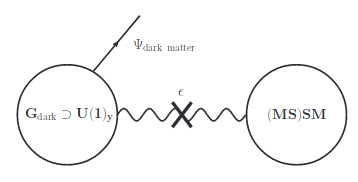
\includegraphics[width=0.4\textwidth]{Fisica_de_Particulas/imagenes/sketch_darksector.png}
    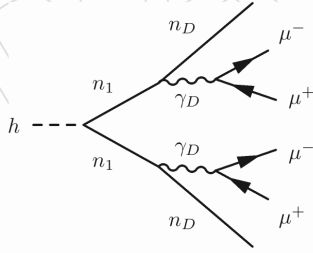
\includegraphics[width=0.4\textwidth]{Fisica_de_Particulas/imagenes/darksusy_feynman.png}
    \caption{ Ilustración esquemática de la conexión entre el sector oscuro y el modelo estándar, los cuales están conectados mediante un término de mezcla dinámica.}
    \label{fig:sketch_darksector}
\end{figure}



Las expresiones para los anchos parciales permiten el cálculo del tiempo de vida del fotón oscuro:
\begin{eqnarray}
\label{an-15-455:ec6}
\tau_{\gamma_D} = \dfrac{}{\Gamma_{\gamma_D Total}} =\dfrac{1}{\Gamma_{\gamma_D \rightarrow e^+ e^-} + \Gamma_{\gamma_D \rightarrow \mu^+ \mu^-} + \Gamma_{\gamma_D \rightarrow hadrons }}
\end{eqnarray}
El tiempo de vida está directamente relacionada con el parámetro $\epsilon$ y la masa del fotón oscuro se obtiene:
\begin{eqnarray}
\label{an-15-455:ec7}
\tau_{\gamma_D}(\epsilon,m_{\gamma_D}) =\dfrac{1}{\epsilon^2}\times f(m_{\gamma_D})
\end{eqnarray}
Es conveniente representar el tiempo de vida $\tau_{\gamma_D}$ en unidades de distancia $c\tau_{\gamma_D}$, donde $c$ es la velocidad de la luz. También es conveniente medir $c\tau_{\gamma_D}$ en milímetros porque la sensibilidad del análisis a esta variable es $\sigma(mm)$. Las restricciones sobre $\epsilon$ y la masa del fotón oscuro podrían obtenerse a partir de las restricciones sobre la vida útil del fotón oscuro porque están directamente relacionadas entre sí, como ya se comprobo anteriormente.

El diagrama de Feynman del proceso del SUSY oscuro  $h \rightarrow 2n_1 \rightarrow 2n_D + 2\gamma_D \rightarrow 2n_D + 4\mu$ se muestra en la Fig. \ref{fig:sketch_darksector}. Este modelo de referencia es solo un escenario posible, y se elige como una representación única de un rango muy amplio de espacio de parámetros disponibles. Este modelo simple del sector oscuro se puede ampliar de varias maneras; versiones más complejas involucran otros bosones oscuros de Higgs, $W$ y $Z$. También hay muchos otros procesos permitidos, como por ejemplo $pp \leftarrow h \leftarrow Z_D Z / Z_D Z_D / Z_a \leftarrow 4\mu$. En este análisis representamos los resultados de una manera que permite reinterpretaciones adicionales en el marco de otros modelos.a





Entre sus observaciones más recientes \ref{anexoA} se ha reportado un flujo de positrones anómalo que tiene una posible explicación en el proceso de aniquilación de partículas de materia oscura, donde se libera energía en forma de positrones. Dicho flujo anómalo puede observarse
a partir de los 25 GeV en la Figura \ref{fig:AMS_positronflux} donde también se presenta una comparación con otros experimentos que observan similar comportamiento.

\begin{figure}[ht!]
    \centering
    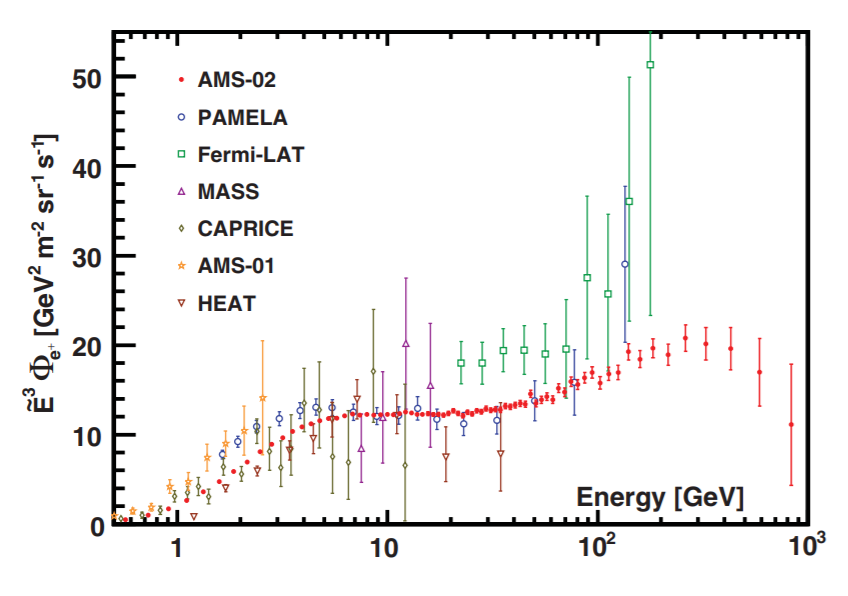
\includegraphics[width=0.75\textwidth]{Fisica_de_Particulas/imagenes/AMS_positronflux.png}
    \caption{Flujo de positrones medido por el experimento AMS-02, comparado con los experimentos PAMELA, Fermi-LAT, MASS, CAPIRCE, AMS-01 y HEAT.}
    \label{fig:AMS_positronflux}
\end{figure}

Estas observaciones cosmológicas han motivado a los físicos teóricos de altas energías a postular nuevos modelos en los cuales la composición de la materia oscura se pueda entender por medio de nuevas partículas elementales no descritas en el modelo estándar y que sin embargo podrían estar siendo producidas en los aceleradores de partículas modernos como el Gran Colisionador de Hadrones en Ginebra, Suiza. Los modelos propuestos se encuentran en la categoría que se conoce como extensiones al modelo estándar y por lo general involucran la existencia de nuevas partículas cuyas fuerzas e interacciones están descritas por alguna variación de la teoría cuántica de campo, lo que sugiere que sus mecanismos de producción y propiedades pueden ser estudiados por el formalismo de la física de partículas y la parte experimental por medio de los detectores de partículas con métodos de recolección de datos, selección de eventos y técnicas estadísticas para el análisis y extracción de posibles señales.

\subsection{Formulación Teórica}

%Se sabe que el modelo estándar proporciona una descripción incompleta de la física de partículas y una serie de extensiones del \ME ~ predicen la existencia de nuevos bosones de luz. Un posible modelo de búsqueda independiente para la producción en pareja de un bosón ligero que se descompone en un par de muones. 

%Un ejemplo simple de producción de pares en colisiones protón-protón (pp) es $pp \rightarrow h \rightarrow 2a + \chi \rightarrow 4\mu + \chi$, donde $h$ es un bosón de Higgs, a es el nuevo bosón neutro ligero, y X son partículas de espectador que se predicen en varios modelos. Si bien la producción a través del bosón h es posible, no se requiere en la búsqueda presentada aquí: el único requisito es que un par de bosones de luz idénticos sean vértices comunes de datos y un bosón de luz de decaimiento se descomponga posteriormente en un par de muones. Estos pares de muones se denominan ``dimuones'', el vértigo y los nuevos vértices de producción de bosones ligeros pueden ser desplazados. La naturaleza genérica de esta firma significa que cualquier límite establecido en el producto de la sección transversal, la fracción de ramificación a los dimuons al cuadrado, y la aceptación es independiente del modelo; Por lo tanto, puede ser reinterpretado en el contexto de modelos específicos.









